% Overleaf entry point: compile with pdfLaTeX (TeX Live 2025 or newer).
\pdfminorversion=4
\pdfobjcompresslevel=0
\documentclass[11pt,letterpaper]{article}
\usepackage[margin=0.88in,headheight=15pt,footskip=28pt]{geometry}
\usepackage[T1]{fontenc}
\usepackage{newtxtext,newtxmath}
\usepackage{microtype,graphicx,booktabs,tabularx,array,amsmath,xcolor}
\usepackage{enumitem,caption,fancyhdr,titlesec,natbib,url,xurl,placeins,flafter,needspace}
\usepackage[colorlinks=true,linkcolor=ink,citecolor=ink,urlcolor=accent]{hyperref}
\definecolor{ink}{HTML}{203543}
\definecolor{accent}{HTML}{215B79}
\definecolor{muted}{HTML}{64737D}
\setlength{\parindent}{1.15em}
\setlength{\parskip}{3pt}
\linespread{1.065}
\setlength{\emergencystretch}{2em}
\widowpenalty=10000
\clubpenalty=10000
\brokenpenalty=10000
\AddToHook{cmd/section/before}{\Needspace{7\baselineskip}}
\setcounter{topnumber}{3}
\renewcommand{\topfraction}{.9}
\renewcommand{\textfraction}{.08}
\renewcommand{\floatpagefraction}{.8}
\captionsetup{font=small,labelfont=bf,labelsep=period,justification=raggedright,singlelinecheck=false}
\titleformat{\section}{\large\bfseries\color{ink}}{\thesection}{.7em}{}
\titleformat{\subsection}{\normalsize\bfseries\color{ink}}{\thesubsection}{.6em}{}
\titlespacing*{\section}{0pt}{15pt}{7pt}
\titlespacing*{\subsection}{0pt}{10pt}{4pt}
\pagestyle{fancy}\fancyhf{}
\fancyhead[L]{\small\textsc{Low-cost extraction of economic forecasts}}
\fancyhead[R]{\small\color{muted}Research manuscript}
\fancyfoot[C]{\small\thepage}
\renewcommand{\headrulewidth}{.3pt}
\setlist{nosep,leftmargin=*}
\graphicspath{{figures/}}
\newcommand{\note}[1]{\par\vspace{3pt}{\footnotesize\textit{Notes:} #1\par}}
\newcommand{\evidence}[1]{\textsuperscript{\hyperref[app:evidence]{[#1]}}}
\newcommand{\pathcode}[1]{{\footnotesize\path{#1}}}
\hypersetup{pdftitle={Low-Cost Extraction of Economic Forecasts from Newspapers},pdfsubject={Human validation, measurement sensitivity, and predictive applications},pdfkeywords={historical expectations, newspapers, language models, measurement, forecasting}}

\begin{document}
\thispagestyle{plain}
\begin{center}
{\small\sffamily\color{accent}ECONOMIC MEASUREMENT AND TEXT AS DATA}\par\vspace{11pt}
{\LARGE\bfseries\color{ink}Low-Cost Extraction of Economic\\[3pt] Forecasts from Newspapers}\par\vspace{9pt}
{\large Human Validation, Measurement Sensitivity,\\and Predictive Applications}\par\vspace{12pt}
{\small Research manuscript\enspace$\vert$\enspace Revised October 22, 2026}
\end{center}
\vspace{3pt}
\begin{abstract}
Newspapers preserve economic expectations whose target, timing, and attribution must be interpreted before a forecast can be evaluated. This paper studies inexpensive structured extraction using ProQuest exports for 1900--2010 and a separate exploratory extension for 2011--2026. The historical corpus contains 274,070 machine-verified candidates, with 175,855 scored under deterministic rules; the modern extension contains 91,118 retained candidates, with 56,886 mature, supported claims evaluated. Separate Library of Congress development experiments project API costs of \$26.82 versus \$403.70 for 23,000 pages, with respective F1 scores of 0.636 and 0.784 against a 52-claim model-adjudicated reference. These are development comparisons, not ProQuest production costs or human quality estimates. Two human reviewers evaluated the same 300 sampled candidates: 250 historical and 50 modern. Their decisions are preserved separately; inter-reviewer agreement has not yet been calculated. Existing first-review field comparisons reveal weaknesses in horizons and geographic scope. The central historical result is measurement sensitivity: on 9,260 matched employment claims, article-weighted accuracy ranges from 34.2\% to 57.6\% across outcome bands, while changing the employment benchmark reverses the baseline-relative point estimate. In the modern extension, a frozen recurrent model achieves AUC 0.738 versus 0.654 for a metadata-plus-history logistic control, but paired block intervals do not establish the Brier-score improvement and employment AUC is only 0.306. Modern results remain exploratory because prior outcome exposure is undocumented. The evidence supports inexpensive extraction as candidate generation whose economic use requires human source review, explicit targets, matched baselines, and chronological evaluation.
\end{abstract}
\noindent{\small\textbf{Keywords:} historical expectations; newspaper forecasts; language models; text measurement; forecast evaluation.}
\vspace{4pt}



% Main paper
\section{Introduction}
Economic expectations matter before they become survey responses or numerical forecasts. A newspaper may report a business leader anticipating recovery, an economist expecting unemployment to rise, or an editorial predicting a decline in prices. Such statements can preserve the direction, uncertainty, and attribution of expectations at a particular date. Their historical value is considerable, but turning them into comparable observations requires more than locating future-tense language. A statement about slower growth differs from a prediction of falling output; a forecast about jobs differs from a forecast about the unemployment rate; and a broad outlook may not specify an endpoint that can be scored mechanically.

Language models make it feasible to generate structured candidates from large text collections at relatively low marginal API cost. Whether those candidates support economic conclusions is a separate empirical question. Cheap extraction can be useful even when imperfect, but its usefulness depends on the errors it introduces, the evidence available for validating them, and the outcome rule applied downstream. We therefore examine three linked stages: extraction, source interpretation, and evaluation against economic outcomes.

The main application uses the annual ProQuest economy exports for 1900--2010. We retain 274,070 machine-verified candidates without automatically deduplicating identical stripped labels. The primary historical analysis uses only these annual exports; the raw annual candidates form a sensitivity set. A separate Library of Congress (LOC) experiment supplies development evidence about extraction cost and reference agreement. Its pages and economic results never enter the ProQuest estimation sample. A separately authorized 2011--2026 ProQuest extension contains 91,118 retained candidates and evaluates 56,886 mature, supported claims. We report its exploratory transfer results in the main text, with full details in Appendix~\ref{app:modern}; historical and modern estimates remain separate.

The paper makes three contributions. First, it documents a concrete computational cost--quality comparison, including the precision--recall consequences of verification. The most economical illustrated two-stage configuration costs approximately one-fifteenth as much as the higher-recall configuration in the recorded page-scaling exercise. This establishes a development tradeoff, not a universal price advantage or an end-to-end cost estimate for ProQuest. Second, it reports source-review evidence with the sampling frames, field denominators, and reviewer provenance made explicit. Third, it demonstrates that reasonable-looking changes to benchmark definitions can materially alter conclusions about the same historical claims.

The last contribution is the principal economic finding. Under the original employment rule, the matched sample is correct 34.2\% of the time and exceeds an always-improve baseline by 14.2 percentage points. Under sign-only scoring, accuracy reaches 57.6\%, but the advantage is 10.8 points and its block interval includes zero. Replacing falling unemployment with rising payroll employment changes the baseline-relative point estimate from positive to negative. Higher raw accuracy therefore does not, by itself, identify a better interpretation of what the newspaper predicted.

This argument concerns rules implemented in this repository. We do not assert that other researchers routinely use an undocumented defective threshold, nor infer a field-wide failure from a hypothetical example. The manuscript also makes no new mathematical priority claim: the definitions and elementary identities below organize the empirical comparison. The evidence is an observed dependence of economic conclusions on specific, auditable measurement choices.

Predictive models provide an application rather than the criterion for the paper's success. A recurrent model can distinguish correct from incorrect machine-scored claims without proving that the extraction is valid, that recurrence supplies the improvement, or that the model forecasts recessions. A historical aggregate comparison shows a small average gain from newspaper features, but that gain is uncertain and reverses when 2007--2009 evaluation months are omitted. Reporting these limitations is necessary to establish what this dataset currently measures.


\section{Related research and the scope of the contribution}
\subsection{Historical expectations, sentiment, and uncertainty}
Historical forecast interpretation has direct precedents. \citet{mathy2017} quantify contemporaneous and forward-looking assessments in the business press during the Great Depression. Their object is close to ours: what economic observers believed while events unfolded. Our longer annual corpus and automated candidate generation extend the scale of this inquiry; they do not originate the use of historical press statements to study expectations. The contribution here is a documented chain from extraction choices to claim interpretation and baseline-relative outcomes.

The broader text-as-data literature provides the statistical setting \citep{gentzkow2019}. Newspaper-derived constructs need not be explicit forecasts. \citet{bybee2024} extract topical attention from business news and examine its relationship with economic activity, including incremental information beyond conventional indicators. \citet{barbaglia2022} use aspect-specific news sentiment for macroeconomic forecasting. These approaches motivate a demanding comparison with macro-only predictors, but their targets differ from the correctness of an attributable statement. A topic can be informative without containing a forecast; an explicit forecast can be incorrect while revealing a valuable historical belief. No common-data replication against those published signals is attempted here.

Financial-news research supplies another relevant distinction. \citet{tetlock2007} links pessimistic language in a Wall Street Journal column to market behavior. \citet{garcia2013} studies news sentiment and stock-return predictability, finding that the predictive relationship is concentrated in recessions. These studies establish substantive precedents for extracting economically informative language. They do not imply that every negative sentence predicts a price decline, or that a sentiment coefficient measures a newspaper forecaster's accuracy. For our application, the relevant comparison must align the quoted proposition, asset or macroeconomic target, forecast origin, and horizon. A sentiment index and a directional claim may contain related information without being interchangeable measurements.

\citet{baker2016} develop newspaper-based measures of economic policy uncertainty and validate their construction using several forms of evidence, including human readings. Their historical US index reaches back to 1900 \citep{bakerhistorical}. It offers a natural comparison for a long-run newspaper corpus, but measures policy-related uncertainty rather than the correctness of particular forecasts. The documented historical index also uses source-specific normalization and overlapping newspaper sets. That design highlights a limitation of our exports: without a complete article-processing denominator, raw forecast counts cannot be interpreted as a coverage-normalized attention index. We do not estimate a relationship with EPU in this paper; adding its series to a future comparison would require a documented alignment and an explicit account of changing source coverage.

\subsection{Professional forecasts and the meaning of confidence}
The Livingston Survey \citep{philalivingston} and Survey of Professional Forecasters (SPF; \citealp{philaspf}) supply established records of explicitly elicited economic expectations. The former began in 1946 and the latter in 1968. Federal Reserve staff projections are separately available in the Philadelphia Fed's Tealbook/Greenbook datasets \citep{philagreenbook}. These records are potential external comparators, rather than observations included in the newspaper sample or benchmarks already tested here. A valid comparison would harmonize the economic variable, units, target period, release vintage, and information date before evaluating relative performance. Survey response dates, newspaper publication dates, and staff forecast dates need not describe identical information sets. In particular, the staff projections become public only after a five-year lag; their historical forecast date alone does not make their contents an admissible contemporary public predictor.

\citet{campbell2024} examine probabilistic SPF forecasts and find evidence of overprecision, with little evidence of optimistic bias. Their analysis distinguishes confidence in outcomes from the direction of forecast errors and uses an exploration--validation design. This distinction matters for our interpretation of linguistic confidence. An extracted label such as confident or hedged is not an elicited probability distribution. A low directional hit rate therefore does not, by itself, demonstrate overprecision, and confident language cannot be assigned a numerical probability without a separately validated mapping. Conversely, the probability produced by our claim-correctness model concerns whether a machine-scored label will be correct; it is not the probability originally expressed by a historical speaker. We make no claim to reproduce the SPF overprecision result with newspaper labels.

\subsection{Text measurement and extraction validation}
Validation must match the intended construct. \citet{shapiro2020} compare sentiment measures with human ratings and separately investigate economic applications. \citet{grimmer2013} emphasize problem-specific validation of automated text analysis. \citet{loughran2011} demonstrate that general-purpose negative-word lists can misclassify language in financial filings, motivating domain-specific measurement. Their evidence concerns dictionaries and 10-Ks, not our newspaper extractor; its relevance is the need to validate the interpretation assigned to language in its own setting. For the present study, agreement about the text and success at predicting an economic series are separate requirements. A model's association with future production cannot substitute for checking that the source actually made the forecast attributed to it.

Low-cost language-model annotation is itself established research. \citet{gilardi2023} compare ChatGPT classifications with human annotations across several text tasks and document cost advantages in those applications. Our LOC comparison evaluates extraction spans and inclusion decisions, while the ProQuest review evaluates historical economic fields. Neither sample establishes that the same model ranking transfers across domains. The contribution is therefore application-specific evidence, including adverse results, rather than a claim that inexpensive automated annotation is newly possible.

\subsection{Forecast evaluation, revisions, and model selection}
Proper scoring rules provide a foundation for evaluating probabilistic forecasts \citep{gneiting2007}. Brier loss and log loss assess probabilities, whereas directional accuracy evaluates categorical decisions and AUC evaluates ranking. These measures answer different questions. A proper probability score cannot repair an incorrectly defined outcome: the economic target must first correspond to the proposition being evaluated. Likewise, differences in target prevalence make scores from different samples unsuitable as direct measures of a model's improvement. Our comparisons therefore emphasize matched observations, explicit targets, and the same baseline predictions under each stated rule.

Historical prediction also requires careful treatment of data revisions. \citet{croushore1999} explain how real-time vintages differ from later datasets. We distinguish print-time predictor information, labels admitted to model fitting, and revised outcomes used for retrospective assessment. The selected historical macro benchmark reconstructs vintage information for fitting; the claim-correctness exercise uses frozen revised assessment series and a release allowance. These are different evidentiary standards, and we do not describe the latter as a complete recreation of historical real-time forecasting.

Finally, \citet{cawley2010} show how optimization of a finite-sample model-selection criterion can introduce selection bias in reported performance. Chronological separation addresses information ordering, but cannot restore an untouched evaluation sample after its results have influenced analysis choices. This motivates our disclosure of prior outcome exposure and the exploratory status of the saved extension. The concern is selection and interpretation, not a general objection to simulation or to evaluating estimators against known population parameters. Appendix~\ref{app:examples} states that distinction explicitly.


\section{Data, lineage, and the extraction workflow}
\subsection{Historical corpus and analysis population}
The historical newspaper source is ProQuest \citep{proquesthistorical}, with source access and text analysis organized through its TDM Studio environment \citep{proquesttdm}. The received exports, rather than a provider product description, define the actual analysis population. The source consists of 111 annual raw shards and 111 annual machine-verified shards spanning 1900--2010. The archived exports were copied unchanged from the integration repository at commit \texttt{774b68f}. The raw files contain 488,660 candidate claims; the verified files contain 274,070. The latter represent 146,720 article identifiers, including 105,604 articles with at least one retained claim and 41,116 articles represented only by a no-prediction record. These article counts describe the received exports, not the universe of newspaper articles searched or processed.\evidence{H1}

The newspaper families include the New York Times, Wall Street Journal, Los Angeles Times, Chicago Tribune, Washington Post, Boston Globe, Barron's, and Christian Science Monitor, with a small USA Today component. Historical edition labels are consolidated for descriptive paper-family comparisons. Coverage is uneven: verified Wall Street Journal claims begin in 1984, and scored Chicago Tribune coverage ends in 2001. Consequently, differences over time or across publishers can reflect changes in source composition. The corpus should be described as forecasts reported in selected newspapers, not a probability sample of the American press.

\begin{table}[t]
\caption{Historical corpus and deterministic-scoring flow}\label{tab:flow}
\centering\small
\begin{tabularx}{\linewidth}{Xr}
\toprule
Stage or mutually exclusive exclusion & Claims / records\\
\midrule
Raw annual candidate claims & 488,660\\
Machine-verified candidate claims & 274,070\\
\quad Not explicitly US-national & 80,183\\
\quad Topic without a defensible benchmark & 7,894\\
\quad No scorable direction & 3,176\\
\quad Numeric horizon outside 1--24 months & 2,490\\
\quad Outside benchmark coverage & 2,297\\
\quad Unusable horizon label & 2,175\\
\midrule
Scored under the inherited historical rules & 175,855\\
\quad Of which: pre-1919 business claims using an NBER proxy & 1,047\\
Eligible for the claim-correctness model before split purging & 174,808\\
\bottomrule
\end{tabularx}
\note{The six exclusion rows sum to 98,215; 274,070 minus 98,215 equals 175,855. The NBER-proxy row is a subset of scored claims, not another descriptive exclusion. The 41,116 no-prediction export records are not candidate claims. Raw and verified exports are not a fully reconciled processing ledger; their difference is not labeled a measured rejection count. Sources: H1--H2 and P2, Appendix~\ref{app:evidence}.}
\end{table}

Machine verification is an inclusion filter. It is not independent human validation. The inventory contains 696 verified rows with identical exported labels; all are retained. Because the local exports omit quotations and lack a unique claim identifier, distinct passages can share the same categorical labels. Deduplication on those fields alone would impose an unsupported assumption about identity. We instead preserve file, line, publication date, and article linkage.\evidence{H1}

\subsection{Modern extension and evaluation population}
The separate 2011--2026 export contains 91,118 retained candidates. Excluding 19 default-kept verification exceptions leaves 91,099 primary inputs; 33,071 no-prediction records are kept outside the candidate count. Eligibility and maturity rules remove 32,604 unsupported claims, 1,138 claims with unmatured outcomes, and 471 with reference gaps, leaving 56,886 evaluated claims from 23,775 articles. These are saved October 20, 2026 results, with no interpolation of unavailable outcomes. The historical and modern populations are reported separately throughout.\evidence{N1}

Human source review includes 50 modern candidates sampled across all sixteen publication years. That sample assesses extraction and annotation, including candidates without mature economic outcomes; it is not a random subsample of only the 56,886 evaluated claims. The modern predictive exercise applies frozen historical claim models, but undocumented prior outcome exposure prevents describing it as an untouched confirmatory holdout. Appendix~\ref{app:modern} records the dated reference coverage, exclusions, and model comparisons.

\subsection{From article text to an evaluable claim}
The workflow has five steps. Article text is retrieved within the authorized source environment. An extractor proposes forecast spans and structured labels. A verifier evaluates candidates. Permitted categorical information is exported with source-linked addresses, while the original exports are preserved. Finally, explicit eligibility and outcome-availability rules determine which claims enter each analysis. The historical human comparisons identify the original ProQuest labels as GPT-4o mini outputs \citep{openai4omini}; the LOC experiment uses separately named model configurations. Their costs and quality estimates are not interchangeable.\evidence{V1--V2,X1}

\begin{figure}[t]
\centering
\setlength{\fboxsep}{7pt}
\fbox{\begin{minipage}{.92\linewidth}\small
\textbf{Authorized article text}\hfill Source access and publication date\\[4pt]
$\downarrow$\quad Candidate extraction: passage, topic, direction, horizon, scope, attribution\\[4pt]
$\downarrow$\quad Machine verification: retain or reject proposed candidates\\[4pt]
$\downarrow$\quad Frozen categorical export: preserve article and source-row lineage\\[4pt]
$\downarrow$\quad Source review and explicit analysis-eligibility rules\\[4pt]
\textbf{Two distinct outputs:} textual validity and field agreement; economic outcomes under a stated scoring rule
\end{minipage}}
\caption{A workflow with separate textual and economic checks. Human review evaluates sampled candidates; it does not certify every exported row. LOC development evidence attaches to extraction and verification only.}
\label{fig:pipeline}
\end{figure}

The main fields are topic, economic direction, horizon, geographic scope, confidence language, voice, speaker, and current conditions. They serve different purposes. Topic selects a potential outcome series. Scope prevents a regional or foreign forecast from being judged against a national US aggregate. Horizon determines the endpoint. Attribution separates a newspaper's own assessment from a forecast it reports. Confidence describes language and is not a calibrated probability. Present conditions must be distinguished from a prediction even when both appear in the same paragraph.

The inclusion rubric requires a falsifiable claim about future economic conditions. It excludes current or retrospective descriptions, advertisements, generic rules, non-economic promises, and hypothetical scenarios without a committed forecast. Reporting a forecast skeptically does not necessarily erase the forecast, but republishing one after its outcome is known creates a timing problem. These boundaries matter because a hindsight description scored as a forecast can manufacture apparent predictive skill. Source context, rather than categorical labels alone, resolves such cases.

\subsection{What the received data cannot establish}
The local exports do not supply complete article-processing denominators. A rise in claim counts therefore cannot be interpreted directly as greater attention to the economy. It may reflect retrieval coverage, article availability, extraction yield, or verification behavior. Likewise, fewer verified than raw claims do not identify the number of genuine forecasts removed. The raw set is a sensitivity sample under the same scoring rules, not a second human reference standard.

The pipeline preserves retrospective window annotations and verifier prose outside model inputs. Neither is available as an admissible print-time predictor. All reported historical economic estimates exclude old crisis-window exports and LOC claims. The LOC pages used below are retained solely for extraction development, where their crisis-focused selection is itself a limitation.


\section{Extraction cost and development quality}
\subsection{Reference design and metrics}
The separate LOC material comes from Chronicling America \citep{loc}. The LOC comparison uses 16 pages with 52 reference claims, including three pages with no forecasts, plus a distinct set of 44 boundary decisions. The reference was produced by a language model following a written protocol before the tested extractor outputs were available. It is model-adjudicated, not human gold. The boundary set contains 32 exclusion traps and 12 awkward but eligible forecasts. Its accuracy is a separate diagnostic, not an alternative estimate of population precision.\evidence{X1}

For matched extracted spans, precision is $TP/(TP+FP)$, recall is $TP/(TP+FN)$, and $F_1=2TP/(2TP+FP+FN)$. The saved evaluator uses greedy one-to-one containment matching at 0.7. The protocol text instead mentions a Jaccard threshold of 0.6; this documentation inconsistency must be resolved before treating the benchmark as a finalized validation package. We report the metrics produced by the saved evaluation, with that limitation disclosed.\evidence{X1}

Whole-page reference annotation makes false negatives observable within those pages. In contrast, reviewing only extracted positive candidates cannot reveal forecasts the extractor never proposed. This difference explains why the LOC experiment reports recall while the ProQuest human review does not. It does not make the model-produced LOC reference more authoritative than human review; the two designs answer different questions.

\begin{table}[t]
\caption{Recorded LOC development cost--quality comparison}\label{tab:cost}
\centering\small
\begin{tabularx}{\linewidth}{Xrrrrr}
\toprule
Configuration & Precision & Recall & F1 & \$/1,000 & \$/23,000\\
\midrule
Regex baseline & .609 & .269 & .373 & 0.00 & 0.00\\
OSS extraction & .536 & .712 & .612 & 0.98 & 22.65\\
OSS + self-verification & .618 & .654 & .636 & 1.17 & 26.82\\
OSS + Lite verification & .756 & .596 & .667 & 1.89 & 43.52\\
OSS + Flash verification & .931 & .519 & .667 & 4.58 & 105.43\\
Flash, one window & 1.000 & .654 & .791 & 12.62 & 290.36\\
Flash, 8k windows & .844 & .731 & .784 & 17.55 & 403.70\\
\bottomrule
\end{tabularx}
\note{USD per number of LOC \emph{pages}, using the historical report's token-based projections. OSS denotes the archived gpt-oss-120b configuration; Lite and Flash denote the archived Gemini Flash-Lite and Flash configurations. Exact run names are in Appendix~\ref{app:cost}. The reference is 16 pages/52 claims, produced by a model; these are development metrics. Zero regex cost means zero metered language-model API charges. It excludes labor and computing. Costs are not current quotations, invoices, or ProQuest article costs. Source: X1.}
\end{table}

\subsection{The observed tradeoff}
The self-verifying OSS pipeline identifies 34 of 52 reference claims and returns 21 unmatched claims: precision 0.618, recall 0.654, and F1 0.636. Its recorded projection is \$26.82 for 23,000 pages. The Flash 8k-window configuration identifies 38 reference claims with seven unmatched claims, yielding precision 0.844, recall 0.731, and F1 0.784 at \$403.70. The cost ratio is about 15.1, or 93.4\% lower projected API cost for the economical configuration. Four more matched claims and fourteen fewer unmatched claims distinguish these particular outputs; the sample is too small and specialized to establish a general ranking.\evidence{X1}

Cost and F1 are not monotonically related. The one-window Flash configuration has F1 0.791 at a lower projected cost than its 8k-window counterpart, though it has lower recall. On the boundary exercise, the 8k configuration resolves 43 of 44 cases, versus 41 for the one-window configuration and 36 for OSS self-verification. Reporting the one-window result is essential: the \$403.70 configuration is a higher-recall comparison, not the unique F1 leader or an unqualified optimum.

\begin{figure}[t]
\centering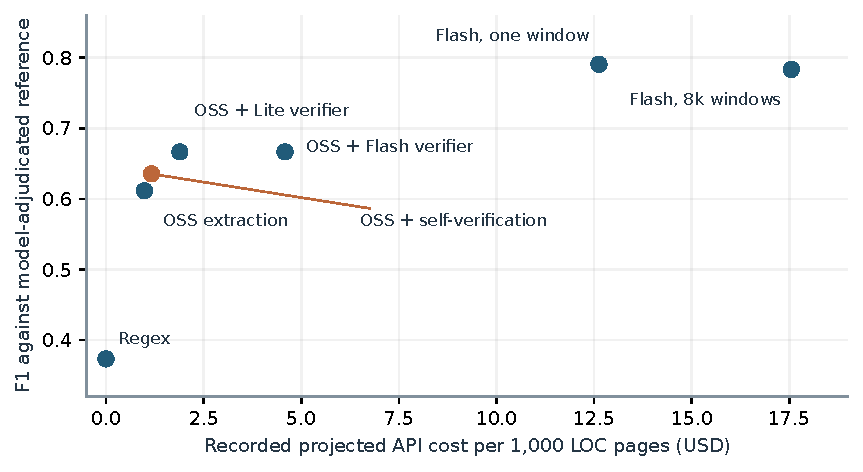
\includegraphics[width=.98\linewidth]{cost_quality.pdf}
\caption{API expenditure and extraction agreement in the LOC development sample. The horizontal axis converts the recorded 23,000-page projections into cost per 1,000 pages. No point represents a ProQuest cost or human-validated F1. The diagram displays observed configurations rather than an estimated population efficiency frontier.}\label{fig:cost}
\end{figure}

Verification changes the composition of errors. Unverified OSS extraction produces 37 true matches and 32 unmatched candidates. Flash verification retains 27 true matches and two unmatched candidates. Precision rises substantially, but ten previously matched claims are lost. A filter cannot recover an omitted candidate unless it also performs a new extraction step. The relevant question is therefore whether reduced false positives justify lost recall for the intended downstream analysis, not whether adding verification is inherently beneficial.

\subsection{Cost accounting and limits to transportability}
For pipeline stages $s$, the recorded projection has the form
\begin{equation}
 C(N)=\frac{N}{16}\sum_s\frac{T_{s,\mathrm{in}}r_{s,\mathrm{in}}+T_{s,\mathrm{out}}r_{s,\mathrm{out}}}{10^6},
 \label{eq:cost}
\end{equation}
where token totals $T$ are measured over the development pages and rates $r$ are the report's historical dollars per million tokens. The formula assumes that token use scales linearly with page count. Different document lengths, retry rates, forecast densities, or output budgets can violate that approximation.

The recorded OSS extraction component is \$22.65 per 23,000 pages. Subtracting it from the rounded pipeline totals gives approximately \$4.17 for self-verification, \$20.87 for Lite verification, and \$82.78 for Flash verification. These are differences of rounded projections, not separately audited bills. The development narrative reports approximately \$0.86 spent on the benchmark, but the cost script sums pipeline costs that reuse extraction stages. Without a reconciled call-level ledger, we cannot certify that figure as unique billed expenditure.\evidence{X1}

Full project cost additionally includes source access, retrieval, failed calls, infrastructure, human review, and interpretation. Local inference removes a provider's per-token charge but does not make hardware, power, or operator time free. No complete ProQuest usage ledger or human-hours record is available in the inspected evidence. Thus, the results support the narrower claim that some extraction configurations have low projected API cost; they do not establish the total cost per valid ProQuest forecast or the savings relative to manual corpus construction.

The reference pages come from a crisis-focused LOC cache. Forecast density, OCR difficulty, publication style, and the mix of advertisements and retrospectives may differ in ordinary periods and in ProQuest articles. The experiment does not establish that those differences leave precision or recall unchanged. A common, human-annotated document sample spanning eras and forecast densities would be needed to test transportability and compare cost per correctly recovered forecast.


\section{Human validation of ProQuest candidates}
\subsection{Sampling and reviewer provenance}
Two human reviewers evaluated the same 300 claims from 299 distinct articles: 250 historical claims and 50 from the modern extension. The author confirmed the first review was completed without AI assistance on October 21, and confirmed both reviewers were human on October 22. Reviewer 2's frozen labels and dated author attestation are preserved separately. The second review protocol records source-only reading without consulting claim-level author labels, machine labels, or realized outcomes; aggregate study summaries had been visible. The first review had mixed machine-label exposure, as detailed below. Inter-reviewer agreement and adjudication have not yet been performed; two completed reviews do not imply a fully blinded design.\evidence{V1--V3}

The original historical batch contains 150 claims from a frame of 175,843 scored verified candidates after excluding 12 pilot records. It retains an initial simple random sample of 100 and adds 50 without replacement from the remaining frame. The initial 100 had prior machine-label exposure; the additional 50 are documented as having machine labels hidden until the annotation was frozen. The second historical batch samples another 100 without replacement from 175,693 remaining eligible addresses. Its findings are shown separately rather than presenting the entire review as an untouched blinded experiment.

The modern batch is stratified by publication year: four records from each of 2011 and 2026 and three from each intervening year. Its frame contains 91,118 retained verified candidates and includes verification exceptions that the predictive analysis later excludes. Unlike the historical frame, these records need not have scorable outcomes. Differences in sample design and eligibility prevent interpreting the pooled 300-record inclusion fraction as a single population validity estimate.

\begin{table}[t]
\caption{First-reviewer inclusion decisions by review batch}\label{tab:review}
\centering\small
\begin{tabularx}{\linewidth}{Xrrrr}
\toprule
Sample & Reviewed & Include & Exclude & Unclear\\
\midrule
Historical batch 1 & 150 & 105 & 44 & 1\\
Historical batch 2 & 100 & 72 & 28 & 0\\
Modern extension & 50 & 35 & 15 & 0\\
\midrule
Reviewed sample total & 300 & 212 & 87 & 1\\
\bottomrule
\end{tabularx}
\note{The total is a record count across different frames, not a pooled population estimate. Historical batches are positive candidates already eligible for legacy scoring; modern sampling covers all retained candidates by year. Source recovery succeeded for sampled records, with documented lineage checks. Sources: V1--V2.}
\end{table}

Inclusion is 105/150 in the original historical batch and 72/100 in the second. The unresolved first-batch case gives a 70.0--70.7\% identification range depending on how that case is classified; this is not a confidence interval. The modern sample includes 35/50 candidates. The saved inverse-inclusion-probability ratio estimate is 73.4\% for its modern frame, versus the unweighted 70.0\% sample fraction. No design-based interval is supplied for that weighted point estimate, and none is invented here.

Reviewer 2 includes 171 of the 250 historical candidates and excludes 79; among the 50 modern candidates, 33 are included and 17 excluded. The second review therefore contains 204 include and 96 exclude decisions. These are descriptive counts from the frozen manifest, not an agreement calculation: matching aggregate counts would not establish that reviewers accepted the same claims. The two sets of judgments remain separate, with no adjudicated consensus or second-reviewer population-weighted estimate asserted here.\evidence{V3}

\subsection{Field agreement and practical usability}
The field-agreement results below compare machine labels with the first human reviewer and are conditional on that reviewer's inclusion decisions. They are not human--human agreement estimates. Table~\ref{tab:fields} reports exact numerator and denominator pairs, because excluding invalid candidates changes the population to which the field rates apply. The historical review shows stronger topic and direction agreement than horizon and scope agreement. In the modern included subset, topic and direction each match on 29/35 claims, horizon on 26/35, and scope on 24/35. These comparisons support using the extraction to organize candidate material, but also identify consequential interpretation errors.

\begin{table}[t]
\caption{Machine--first-reviewer field agreement among included claims}\label{tab:fields}
\centering\small
\begin{tabularx}{\linewidth}{Xrrr}
\toprule
Field & Historical 1 & Historical 2 & Modern\\
\midrule
Topic & 90/105 (85.7\%) & 66/72 (91.7\%) & 29/35 (82.9\%)\\
Direction & 94/105 (89.5\%) & 60/72 (83.3\%) & 29/35 (82.9\%)\\
Horizon & 66/105 (62.9\%) & 49/72 (68.1\%) & 26/35 (74.3\%)\\
Scope & 65/105 (61.9\%) & 49/72 (68.1\%) & 24/35 (68.6\%)\\
Confidence & 75/105 (71.4\%) & 55/72 (76.4\%) & 22/35 (62.9\%)\\
Voice & 79/105 (75.2\%) & 57/72 (79.2\%) & 24/35 (68.6\%)\\
Speaker name & 74/105 (70.5\%) & 43/72 (59.7\%) & 27/35 (77.1\%)\\
\bottomrule
\end{tabularx}
\note{Literal agreement is not always semantic equivalence: name abbreviations can count as mismatches. These are sample summaries, without claimed independent-observation confidence intervals. Current-state agreement is excluded because the original batch used incompatible conventions. Sources: V1--V2.}
\end{table}

\begin{figure}[t]
\centering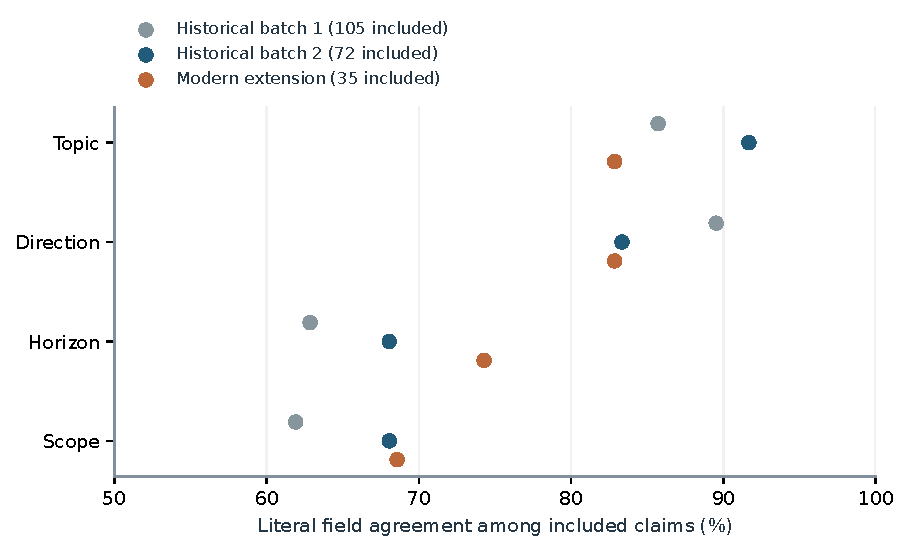
\includegraphics[width=.95\linewidth]{human_agreement.pdf}
\caption{Machine--first-reviewer agreement varies by field and review batch. Displaying the three samples separately preserves their different frames and denominators. Small differences between samples should not be read as statistically established changes over time.}\label{fig:human}
\end{figure}

Several conventions limit interpretation. The review maps approximately four to eight months to six and nine to fifteen months to twelve; annual next-year outlooks also map to twelve. A matching horizon category therefore does not establish an exact endpoint. Speaker-name comparison is literal, so a surname and a full name can disagree while referring to the same person. Price and unemployment fields contain many not-applicable matches; the additional review's applicable-only counts are 12/14 and 4/6, respectively, and are too small to characterize performance broadly.

The original current-state field cannot be pooled with the additional batch. Its saved mismatch reflects differing coding conventions, and the all-eleven-fields match count of 1/105 is consequently not a valid overall accuracy estimate. In the additional batch, all eleven fields match on 6/107 included claims, but even that is exact annotation agreement, not the share of forecasts whose economic outcomes are scored correctly. Joint usability must be defined by the fields needed for a particular estimand, rather than requiring or ignoring fields indiscriminately.

\subsection{What the audit validates}
Four quantities must remain distinct. Inclusion measures whether a proposed passage is a forecast under the review rubric. Field agreement measures whether a retained forecast's annotations match the review. Recall measures whether all genuine forecasts in a document were found. Economic accuracy measures whether a forecast matches its eventual outcome under a specified interpretation. The human sample estimates aspects of the first two; it does not establish the third, and its purpose is not to estimate the fourth.

The review identifies practical error categories: present or past descriptions treated as forecasts, unresolved policy conditionals, generic statements, ambiguous attribution, coarse horizons, and mismatches between geographic scope and the proposed benchmark. The categorical local exports do not provide a consistently coded frequency table for these categories. We therefore discuss them qualitatively and do not invent prevalence estimates or quote restricted source prose. Appendix~\ref{app:examples} supplies explicitly hypothetical examples to clarify the distinctions.

Most importantly, the review does not produce a source-validated strict score for the full corpus. Such a score would require the exact economic quantity, direction, scope, original date, conditionality, and endpoint to be compatible with the outcome rule. The historical estimates below remain estimates for machine-selected, machine-labeled candidates. A global correction using the pooled inclusion fraction would be unjustified because extraction errors can vary with topic, era, horizon, and realized outcome.


\section{Measurement choices and historical forecast evaluation}
\subsection{The scoring contract}
For claim $i$, let $m_i$ denote its publication month, $h_i$ its assigned horizon, $q_i$ its target, and $d_i$ its normalized direction. A scoring specification $s$ maps the target and dates to an outcome $y_i^{(s)}$. Correctness is
\begin{equation}
 z_i^{(s)}=\mathbf{1}\{d_i=y_i^{(s)}\}.
 \label{eq:correct}
\end{equation}
This is a definition of correspondence under an interpretation, not a direct measurement of whether the historical speaker understood the economy. If $q_i$ or $h_i$ misrepresents the passage, $z_i^{(s)}$ can be computed exactly and still answer the wrong substantive question.

The inherited outcome rule compares the publication-month level with the level $h_i$ months later. For production, prices, and markets, the change is $100(X_{m_i+h_i}/X_{m_i}-1)$; for unemployment it is the difference in rate percentage points. The original flat bands are $\pm2\%$ for industrial production, $\pm5\%$ for the nominal Shiller S\&P Composite price series, $\pm1.5\%$ for CPI, and $\pm0.5$ percentage points for unemployment. Changes exactly at a boundary count as flat, subject to the saved numerical tolerance.\evidence{H2}

The core outcome series distributed through FRED are industrial production (INDPRO; \citealp{fredindpro}), the consumer price index (CPIAUCNS; \citealp{fredcpi}), and unemployment (UNRATE; \citealp{fredunrate}). The market outcome uses the Shiller stock-price series \citep{shiller}. Payroll employment (PAYEMS) supplies the alternative employment target \citep{fredpayems}. Recession-state coding draws on USREC and the NBER chronology \citep{fredusrec,nber}; these retrospective labels are outcomes or descriptive classifications, not contemporaneously known forecast features. The saved reference files and their hashes identify the numerical vintages actually used. Bibliographic access dates do not identify or update those frozen snapshots.

The price direction uses the explicit price field. Employment uses the explicit unemployment-direction field when available, otherwise mapping improved employment conditions to falling unemployment. This fallback is operationally convenient but not a semantic equivalence. For business and market claims, improve and worsen map to rising and falling benchmark levels. Shiller prices exclude dividends and are a proxy for broad market statements, not an exact benchmark for every asset forecast. Pre-1919 business claims lack industrial-production endpoints and receive a separate NBER-state proxy in the legacy description; they are excluded from the main sensitivity and claim-model samples.

Positive integer horizons from one to twenty-four months are respected. Vague horizons receive six or twenty-four months when the export records a short or long inference, otherwise twelve months. Invalid numeric horizons and unusable labels are excluded rather than clipped. The verified inventory has 142,810 default-horizon claims, underscoring how frequently source timing is not explicit. Moreover, the scorer's ``stated'' category denotes a numeric machine horizon; it does not guarantee that a human recovered that endpoint from the source.

Within a target-specific sample, article-equal accuracy is
\begin{equation}
 \widehat A_s=\frac{1}{J}\sum_{j=1}^{J}\frac{1}{n_j}
     \sum_{i\in j}z_i^{(s)},\qquad
 \widehat\Delta_s=\frac{1}{J}\sum_{j=1}^{J}\frac{1}{n_j}
     \sum_{i\in j}\left[z_i^{(s)}-\mathbf{1}\{b_i=y_i^{(s)}\}\right],
 \label{eq:paired}
\end{equation}
where $n_j$ counts eligible claims in article $j$, $J$ counts articles, and $b_i$ is the comparison forecast. Both forecasts face identical observations, outcomes, and weights. Equal article weighting limits the influence of articles containing many extracted claims; it does not remove common-month economic dependence.

\subsection{The legacy description and raw sensitivity}
On 175,855 scored historical candidates, claim-weighted correctness is 40.8\%, compared with 53.6\% for the fixed-direction rule that predicts rising production, prices, and stock prices and falling unemployment. The baseline is a target-specific directional comparator, not an optimized universal forecast and not a claim that rising prices improve welfare. Under equal article weights, the rates are 40.9\% and 53.6\%, a gap of $-12.7$ percentage points.\evidence{H2}

The raw sensitivity set, processed under the same deterministic rules but on its own eligible support, has article-weighted accuracy 41.7\% against 55.2\% for the baseline. Its gap is $-13.5$ points. Because verification changes composition, the difference between raw and verified rates is not a causal estimate of the verifier's effect on forecast quality. It does show that replacing the primary candidate set with raw exports does not reverse the negative aggregate comparison in this saved exercise.

These pooled results mix targets, eras, horizons, and benchmark availability. They should not be presented as a single universal historical ``accuracy of newspapers.'' The matched employment exercise below deliberately holds the claims and weights fixed to isolate changes in the outcome definition.

\subsection{Changing the flat band on identical employment claims}
The principal sensitivity cohort contains 9,260 verified employment claims from 7,463 articles with numeric machine horizons and non-NBER benchmark support. It compares three recorded specifications: the original half-percentage-point unemployment band, that band multiplied by $h_i/12$, and a zero-width sign-only band. Duration scaling is a linear sensitivity scenario, not a human-validated correction. Sign-only scoring counts even economically tiny nonzero changes. All three use the same claims and article weights.\evidence{M1}

\begin{table}[t]
\caption{Employment scoring sensitivity on common support}\label{tab:employment}
\centering\small
\begin{tabularx}{\linewidth}{Xrrrr}
\toprule
Scoring rule & Claims correct & Baseline & Gap (pp) & 95\% block interval\\
\midrule
Original & 34.2\% & 20.1\% & +14.2 & [3.5, 25.9]\\
Duration scaled & 43.2\% & 27.2\% & +16.0 & [2.3, 30.0]\\
Sign only & 57.6\% & 46.8\% & +10.8 & [$-7.0$, 26.5]\\
\bottomrule
\end{tabularx}
\note{9,260 identical claims, 7,463 articles. The comparator always predicts improvement, operationalized as falling unemployment. Equal total weight per article within this cohort. Intervals are paired five-year calendar-block bootstrap intervals for the gap: 14 occupied blocks and 5,000 draws, conditional on saved scoring choices. They omit interpretation and specification-selection uncertainty. Source: M1.}
\end{table}

\begin{figure}[t]
\centering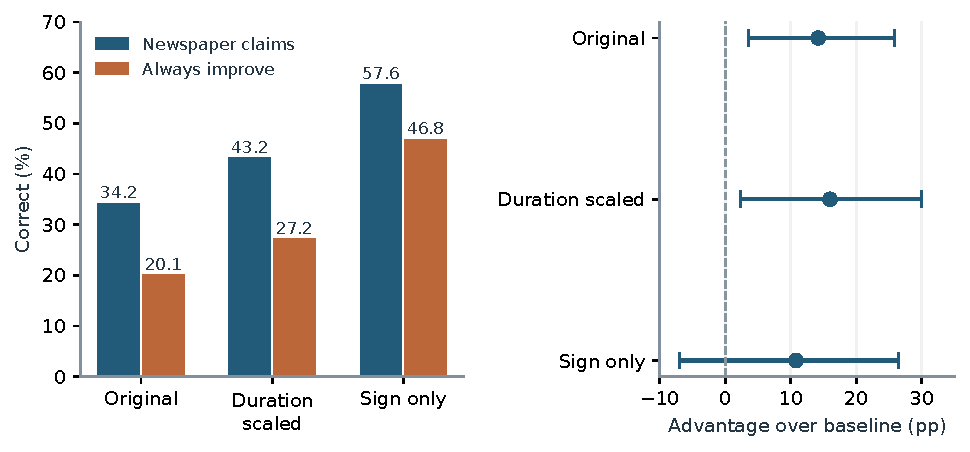
\includegraphics[width=\linewidth]{employment_sensitivity.pdf}
\caption{Higher measured accuracy does not imply a larger advantage over the comparator. Left: claim and baseline correctness under each rule. Right: paired baseline-relative differences with the saved 95\% five-year block intervals. Claims and weights are fixed across specifications.}\label{fig:employment}
\end{figure}

The accuracy increase from 34.2\% to 57.6\% is 23.4 percentage points. Yet the fixed comparator improves by 26.8 points, so the newspaper advantage is smaller under sign-only scoring. The flat-band choice changes which outcomes are common: the always-flat comparator scores 50.6\% under the original rule, 35.2\% under duration scaling, and 5.8\% under sign-only scoring. Under the original band, newspapers underperform always-flat by 16.4 points even though they outperform always-improve. These facts show why reporting only one favorable baseline comparison is incomplete.

The results are descriptive specification sensitivity, not a test that the original band is logically invalid. A tolerance band can be appropriate for a forecast of economically material change. The source might instead commit to any increase, in which case sign-only scoring may be closer. Choosing the rule because it produces the highest hit rate would use outcomes to decide what the forecast meant. Source interpretation should precede that choice.

\subsection{Employment growth and unemployment are different targets}
The alternative-target exercise compares falling unemployment with rising payroll employment on the same 9,260 claims. After orienting both series toward improving labor-market conditions, sign-only outcomes disagree on 21.95\% of article-weighted observations. Employment can grow while the unemployment rate rises, for example if the labor force expands sufficiently. Benchmark disagreement is therefore not automatically a data error. It is evidence that the two economic questions are different.\evidence{M2}

\begin{table}[t]
\caption{Changing the employment benchmark reverses the baseline-relative point estimate}\label{tab:target}
\centering\small
\begin{tabularx}{\linewidth}{Xrrrr}
\toprule
Sign-only outcome & Claims correct & Baseline & Gap (pp) & 95\% block interval\\
\midrule
Unemployment falls & 57.6\% & 46.8\% & +10.8 & [$-7.0$, 26.5]\\
Payroll employment rises & 55.1\% & 63.3\% & $-8.2$ & [$-33.2$, 19.0]\\
\bottomrule
\end{tabularx}
\note{Same 9,260 claims with common endpoint support and equal article weights. Both comparators always predict improving labor-market conditions, mapped to the relevant series. This is an alternative interpretation of broad employment labels, not a source-validated relabeling of every claim. The saved alternative-target exercise also preserves frozen-versus-refreshed-series checks. Source: M2.}
\end{table}

The newspaper hit rate changes only modestly, from 57.6\% to 55.1\%, but the baseline rises from 46.8\% to 63.3\%. The resulting advantage changes by approximately $-19.0$ percentage points. The intervals are wide and include zero for both sign-only comparisons. The robust conclusion is the sensitivity of the point estimates and comparative interpretation, not established newspaper superiority under one target and inferiority under another.

This distinction extends beyond employment. Lower inflation is a decline in the rate of price growth, whereas falling prices are a decline in the price level. Slower output growth can coexist with rising output. A recession onset is an event, whereas an industrial-production endpoint change describes a particular series over a particular interval. An extractor that assigns only a broad topic cannot resolve these meanings by itself.

For fixed claims and weights, an elementary bound clarifies the arithmetic. If the same normalized prediction is scored against two outcome labelings, then
\begin{equation}
 |\widehat A_s-\widehat A_{s'}|
 \leq \frac{\sum_i w_i\mathbf{1}\{y_i^{(s)}\neq y_i^{(s')}\}}{\sum_i w_i}.
 \label{eq:bound}
\end{equation}
Only observations whose outcome labels change can change correctness. This follows directly from the indicator definition and is not offered as a novel theorem. It also does not establish which labeling is right. For a baseline-relative gap, both the claim and comparator terms can change; under the same fixed prediction mapping the analogous bound is twice the weighted disagreement. The empirical task remains identifying the economic proposition in the source.

\subsection{Dependence, uncertainty, and selection}
Claims are not independent economic trials. Multiple articles can discuss the same month, and overlapping horizons share much of the same outcome path. The primary historical sensitivity intervals therefore resample occupied five-year publication blocks in pairs, preserving model or rule comparisons within a block. Two- and ten-year versions are retained in the saved outputs. The employment analysis has 14 occupied five-year blocks; thousands of claims do not create thousands of independent business-cycle realizations.

These intervals condition on the saved observations, interpretations, and fitted outputs. They do not capture uncertainty about source validity, target choice, or the process that selected specifications after earlier results were inspected. The publication specification was written after historical analyses had been viewed. It is not a preregistration, and the sensitivity analyses do not create a fresh holdout. We consequently report their magnitudes and stability rather than promote a winning rule from observed performance.


\section{Predictive applications: historical and modern evidence}
\subsection{Predicting correctness of an extracted claim}
The first predictive task estimates $P(z_i^{(s)}=1\mid\mathcal I_i)$, where $z_i^{(s)}$ is the deterministic correctness label and $\mathcal I_i$ contains permitted information at publication. This is a forecast of claim correctness under the scoring contract. It is neither the probability that extraction is valid nor the probability of a recession.

The frozen recurrent model uses the previous twelve complete calendar months of national forecast distributions across four topics. Each topic contributes five normalized direction shares, log claim count, and an observed-coverage indicator. Current-claim inputs are topic, paper family, voice, hedging category, direction, horizon basis, and numeric horizon. The current publication month is excluded from the sequence. No quotation text, speaker identity, realized outcomes, prior hit rates, crisis annotations, verifier prose, NBER state, or macro reference value enters as a feature. Log counts describe export volume, not a normalized attention measure.\evidence{P2}

A one-layer, 24-unit gated recurrent unit (GRU) feeds a 32-unit head with 15\% dropout. Predictions average three preset seeds. Training publications precede 1985; validation spans 1985--1994; final historical evaluation spans 1995--2010. Outcomes are purged from earlier splits unless their endpoint plus a three-month allowance precedes the next split. After 7,743 purged claims, the split counts are 70,722 training, 39,536 validation, and 56,807 evaluation claims. Preprocessing is fitted on training data only; validation log loss selects epochs.

\begin{table}[t]
\caption{Historical claim-correctness prediction, 1995--2010}\label{tab:rnn}
\centering\small
\begin{tabularx}{\linewidth}{Xrrrr}
\toprule
Model & AUC & Average precision & Brier & Log loss\\
\midrule
Training-prevalence constant & .500 & .409 & .244 & .681\\
Metadata logistic & .678 & .579 & .218 & .629\\
Metadata + history logistic & .634 & .596 & .236 & .692\\
Frozen GRU ensemble & .761 & .683 & .193 & .565\\
\bottomrule
\end{tabularx}
\note{Equal article weights; 56,807 claims. Correctness prevalence is .409. Binary Brier has range 0--1 and lower is better; AUC and average precision measure discrimination. These saved development comparisons do not establish a universally superior model. Source: P2.}
\end{table}

The ensemble's average-precision advantage over the metadata-plus-history logistic control is 0.0876, with a saved five-year block interval of $[-0.1912,0.2102]$ based on four blocks and 400 draws. Separate saved block-swap tests of Brier differences also fail to establish superiority after the reported adjustment. The small number of time blocks sharply limits inferential resolution. Moreover, the logistic comparison does not isolate recurrence from nonlinear function approximation; a matched feed-forward neural control has not been supplied.

Although features respect publication ordering, outcome labels use frozen revised historical series. A three-month release allowance alone cannot prove that every revised value was known then. Modern language models used for historical extraction can also contain later knowledge in their pretrained parameters. Restricting the prompt to source text reduces overt hindsight use but does not certify its absence. This exercise is chronological prediction from reconstructed historical features, not a claim that the entire modern extraction system could have operated in 1900.

\subsection{Modern transfer of frozen claim models, 2011--2026}
On 56,886 mature, supported modern claims, the frozen baseline GRU achieves article-weighted AUC 0.738 and Brier loss 0.1770, compared with AUC 0.654 and Brier loss 0.1936 for the metadata-plus-history logistic control. The Brier improvement is 0.0165, with a paired five-year block interval of $[-0.0092,0.0376]$. Thus the point estimates favor the recurrent model, while the interval does not establish a stable improvement. The GRU with both political separation and forecast disagreement attains AUC 0.749, also without an established incremental Brier gain. No models are selected or recalibrated on these modern results.\evidence{N1}

Transfer is strongly topic-dependent: baseline-GRU AUC is 0.906 for prices, 0.788 for markets, 0.767 for general business, and 0.306 for employment. These outcomes concern correctness under the existing scoring contract, not the validity of extracted passages. Undocumented prior modern outcome exposure, calibration weaknesses, and the employment failure limit the generalization claim. Appendix~\ref{app:modern} supplies all model metrics, calibration results, and the separate monthly downturn exercise. None of these modern claims is pooled into the historical measurement-sensitivity estimates.

\subsection{Incremental information for aggregate production}
The second task predicts a six-month industrial-production direction from month $t-1$ to $t+5$, with an inclusive $\pm2\%$ flat band. Its unit is a monthly forecast origin. It compares a selected macro-only model with the same model augmented by four newspaper signals: recent net direction, common-paper change, disagreement, and cross-paper dispersion. A recent class-frequency comparator is retained.\evidence{P1}

The core evaluation covers 408 months from January 1977 through December 2010. Each January, training-only forward validation chooses among twelve combinations of macro feature set, regularization strength, and expanding versus recent-120-month estimation windows. Macro features are production growth alone or production growth plus unemployment change. Historical label vintages are used at inner and outer refits. The press-augmented regression inherits the macro-selected settings and training months; it is not retuned to maximize its evaluation gain. The procedure was nevertheless designed after inspection of an earlier historical comparator, so the reported period is not untouched.

Multiclass Brier loss is the sum of squared errors over fall, flat, and rise and ranges from zero to two. Macro-only Brier is 0.6327, compared with 0.6228 for macro plus press and 0.6443 for recent class frequencies. The primary improvement, macro-only minus macro-plus-press loss, is 0.0099. Its paired five-year block interval is $[-0.0637,0.0808]$, with seven calendar blocks. Log loss falls from 0.9989 to 0.9606, and accuracy rises from 35.8\% to 44.1\%; these descriptive gains do not remove uncertainty in the primary comparison.

When the already-inspected 2007--2009 scoring months are omitted, 372 months remain. Macro-only Brier is 0.6164 and macro-plus-press Brier is 0.6214, an improvement of $-0.0050$. This is a scoring exclusion using the saved forecasts, not a new fit and not evidence from excluded crisis-window exports. It shows that the average gain is sensitive to a particular evaluation episode. The manuscript therefore does not claim a stable incremental forecasting advantage across eras.


\section{Discussion}
The results identify where inexpensive extraction is most immediately useful. It can generate a large, source-linked candidate collection; support targeted review by topic, horizon, and scope; and enable explicit sensitivity analysis. Those capabilities are substantive even when extraction is imperfect and predictive superiority is unproven. The key restriction is that the candidate corpus should not be described as a uniformly validated set of historical forecasts.

Cost and validity are separate dimensions of that judgment. The LOC experiment shows that low projected API expenditure need not imply zero extraction capability. It also shows a real error tradeoff: the economical self-verifying configuration has more unmatched claims and fewer reference matches than the higher-recall configuration. The ProQuest human review then establishes that inclusion and field agreement require further attention in the actual economic domain. Because the experiments differ in source, task, and reference construction, we cannot combine their cost and quality numbers into a single cost-per-valid-claim estimate.

The central measurement result is stronger than a generic warning about noisy labels. On a fixed historical cohort, observed accuracy, baseline accuracy, and their difference respond differently to the scoring rule. Switching the employment benchmark changes the sign of the estimated relative advantage without dramatically changing the newspaper hit rate. This illustrates why a paper about forecast accuracy must state both the proposition being judged and the comparison forecast. A favorable raw percentage is insufficient evidence of skill.

Several limitations remain consequential. Retrieval coverage and missing processing denominators restrict representativeness. The positive-candidate audit leaves recall unknown. Two human reviews are now available, but inter-reviewer agreement and adjudication remain unmeasured; partial machine-label exposure and coarse horizon categories also limit conclusions about annotation reliability. Revised outcome data and modern pretrained extraction limit claims of historical real-time feasibility. Block intervals have few independent units and omit extraction and model-selection uncertainty. The separate modern extension adds evidence about transfer but includes prior-exposure uncertainty, uneven calibration, and a pronounced employment failure (Appendix~\ref{app:modern}).

The next study should address these limits directly. The existing two-reviewer candidate audit should be extended to a shared sample of complete documents, including documents without forecasts, before comparing inexpensive and expensive extractors. That design would measure recall, inclusion precision, field agreement, and adjudication uncertainty on common support. A call-level usage ledger and review-time record would permit full cost accounting. For economic validation, source-supported targets and endpoints should be fixed before inspecting realized correctness, followed by matched-baseline estimates for the audited population. Any broader error adjustment would require a documented sampling design and assumptions about how reviewed and unreviewed records relate.

Prospective evaluation should freeze preprocessing, target definitions, model candidates, and forecast publication times before outcomes mature. Such an exercise would test performance under a genuinely new sequence of economic events. The present results do not justify a causal effect of political polarization, the supremacy of recurrent networks, or a successful 2026 recession forecast. They justify a research program in which inexpensive extraction expands the observable historical record while source validation and explicit economic definitions constrain the conclusions drawn from it.


\section{Conclusion}
Low marginal extraction cost can make a large collection of historical economic statements computationally accessible. The evidence here demonstrates that possibility in a limited development comparison and documents substantial human-review work on the ProQuest application. It also shows why extraction success alone is insufficient: interpretation choices change the outcomes against which forecasts are judged, the strength of simple baselines, and sometimes the sign of the estimated advantage over those baselines. The separate 2011--2026 extension demonstrates transfer of the frozen pipeline to modern candidates, alongside uncertain predictive gains and a severe employment failure. A useful expectations dataset therefore requires affordable candidate generation, traceable source judgments, and a transparent scoring contract across both periods. The paper's principal finding is that these stages must be evaluated together while their distinct evidentiary roles remain visible.


\section*{Data, reproducibility, and disclosure}
This manuscript synthesizes saved economic results through October 20, 2026 and reviewer-provenance updates through October 22, 2026. No new extractor, economic scorer, or predictive model was fitted for the paper. Publication figures are regenerated from saved summaries, and Appendix~\ref{app:evidence} maps empirical claims to exact repository files. Historical annual source exports remain unchanged; identical stripped labels are retained. Source prose and contextual notes requiring ProQuest access remain in the authorized environment. The manuscript does not assert public redistribution rights for those materials.

Human-review provenance follows the author's October 21 correction that the first review was completed without AI assistance and October 22 confirmation that two human reviewers evaluated the same 300 claims. Reviewer 2's frozen decisions are now included as separate descriptive counts. Inter-reviewer agreement has not been calculated, and complete blinding is not asserted. AI assistance was used to assemble and draft this manuscript. Authorship, affiliations, funding, and conflict disclosures are reserved for the actual authors.



\FloatBarrier
\appendix
\section{Separate modern extension: saved exploratory evidence}\label{app:modern}
The following results reproduce the separately authorized October 20, 2026 extension specified in the dated modern-analysis amendment. They are not new analyses for this manuscript and are not pooled with the annual 1900--2010 estimates. Prior modern outcome exposure remains undocumented, so the extension is exploratory rather than an untouched confirmatory holdout. This distinction holds even though the saved claim models were frozen and their historical predictions were reproduced before application.\evidence{N1--N2}

\subsection{Intake, maturity, and frozen claim models}
The intake has 91,118 retained candidates. Removing 19 default-kept verification exceptions leaves 91,099 primary inputs; 33,071 no-prediction records are separately excluded from inputs. The source exports retain their original bytes and row addresses. Of the primary candidate inputs, 32,604 lack supported scope, topic, direction, or horizon; 1,138 are unmatured; and 471 have reference gaps. The evaluated set therefore contains 56,886 mature, supported claims from 23,775 articles. Missing outcomes are not interpolated.

The modern claim models use unchanged historical fitted parameters. The deterministic outcome rules retain a three-month maturity allowance as of October 20, 2026. The saved reference run records failed refresh attempts and uses preserved snapshots, including production, CPI, and unemployment through June 2026. This is a dated evaluation, not a claim that the manuscript refreshed all economic series to its preparation date.

\begin{table}[t]
\caption{Modern claim-correctness prediction: frozen baseline and secondary arms}\label{tab:modern}
\centering\small
\begin{tabularx}{\linewidth}{Xrrrr}
\toprule
Model & AUC & Brier & Log loss & Accuracy\\
\midrule
Metadata logistic & .662 & .1983 & .5861 & .6987\\
Metadata + history logistic & .654 & .1936 & .5789 & .7223\\
Frozen GRU, baseline & .738 & .1770 & .5347 & .7539\\
GRU + political separation & .692 & .1826 & .5503 & .7618\\
GRU + forecast disagreement & .712 & .1819 & .5479 & .7388\\
GRU + both measures & .749 & .1742 & .5259 & .7610\\
Historical 8-unit challenger & .723 & .1775 & .5792 & .7743\\
\bottomrule
\end{tabularx}
\note{56,886 common claims, equal article weights. Positive correctness prevalence is .2868. The historical challenger is disclosed without promotion. Accuracy uses a .5 decision threshold; a classifier always predicting incorrect would attain .7132 accuracy from the evaluated prevalence, so accuracy alone is not a strong skill diagnostic. Source: N1.}
\end{table}

The primary GRU's Brier improvement over metadata-plus-history logistic is 0.0165, with a paired five-year block interval of $[-0.0092,0.0376]$. The baseline GRU minus the both-measures GRU yields an improvement of 0.0028 for the added inputs, with interval $[-0.0058,0.0191]$. These intervals do not establish the primary gains. The simpler metadata-only comparison has an interval favoring the GRU, but it is a weaker information-set comparator and does not override the primary comparison. There are four occupied blocks with 17,784, 18,017, 21,072, and only 13 claims, respectively. The nominal block count overstates the amount of balanced temporal replication.

Political separation and forecast disagreement measure different constructs. The former uses prior House rollcalls, averaging the absolute Democratic--Republican difference in actual yes-vote shares over a twelve-month window ending two months before the origin. The latter averages $4p_+p_-$ over three completed print months for business claims, with documented coverage rules. It measures opposing directional camps, not newspaper political ideology. Both are lagged; retrospective database curation remains different from archived real-time releases. Neither predictive association identifies a causal effect of polarization.\evidence{P3}

\subsection{Calibration and topic failure}
Discrimination varies substantially. The primary GRU's modern AUC is 0.906 for prices (6,750 claims), 0.788 for markets (9,234), 0.767 for general business (33,509), and 0.306 for employment (7,393). Employment Brier is 0.2707. AUC below 0.5 indicates that the saved ranking is reversed relative to the correctness label in that subgroup; it does not establish that employment forecasts themselves have an accuracy of 30.6\%, nor license post hoc reversal of the model as a validated remedy.

\begin{figure}[t]
\centering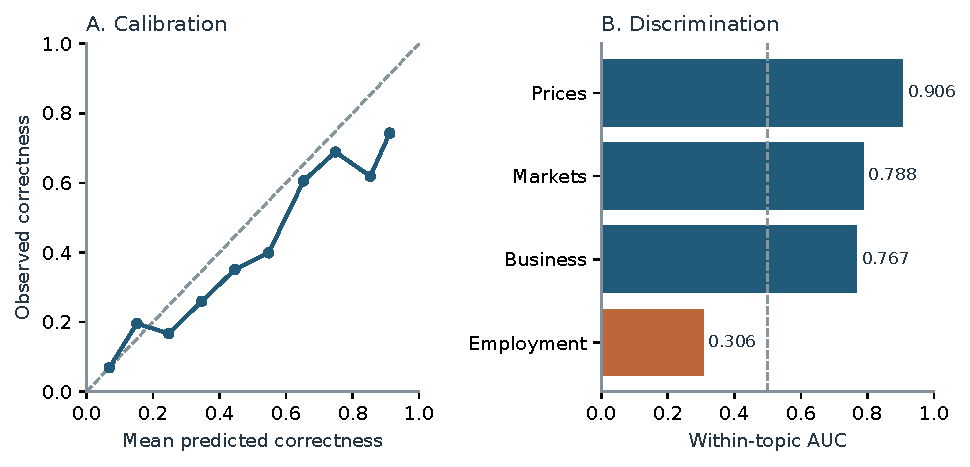
\includegraphics[width=\linewidth]{modern_diagnostics.pdf}
\caption{Saved modern diagnostics for the primary frozen GRU. Panel A uses the saved article-weighted calibration bins; the diagonal is perfect calibration. Panel B displays topic-specific AUC, with the .5 reference marked. Pooled performance conceals substantial employment failure and overconfidence in several probability bins. Source: N1.}\label{fig:modern}
\end{figure}

Calibration also limits interpretation. In the .8--.9 bin, mean predicted correctness is .853 but observed correctness is .619 across 2,168 claims. In the highest bin, the corresponding values are .912 and .743 across 474 claims. These are saved weighted bin means with unweighted claim counts, not independent-bin inference. They demonstrate why an AUC of .738 should not be translated into well-calibrated probabilities. No evaluation-set recalibration is introduced in this manuscript.

\subsection{Separate monthly downturn models}
The downturn exercise uses separately fitted monthly logistic models. Its recession-onset target is any transition from nonrecession to recession in months $t$ through $t+11$; an already ongoing recession is not a new onset. Its production-decline target compares industrial production at $t+11$ with $t-1$. The main production target is any decline, with a greater-than-2\% sensitivity. These are distinct from claim correctness and from the historical six-month, three-class macro target.

Five candidates per target comprise an expanding, Laplace-smoothed event base rate and four ridge logistic variants: press only, press plus political separation, press plus forecast disagreement, and press plus both. Annual January refits admit only mature prior outcomes, using a 24-month allowance for recession dating and three months for production. Candidate selection uses pre-2011 rolling Brier results and remains fixed for modern evaluation. Revised assessment outcomes and reconstructed vote data mean this is not a complete vintage-real-time exercise.\evidence{N2}

\begin{table}[t]
\caption{Modern downturn evaluation against the event base rate}\label{tab:downturn}
\centering\small
\begin{tabularx}{\linewidth}{Xrrr}
\toprule
Target and selected model & Origins & Brier & Base-rate Brier\\
\midrule
Recession onset; press + both & 154 & .0696 & .0832\\
Any production decline; press + forecast disagreement & 175 & .2272 & .2570\\
\bottomrule
\end{tabularx}
\note{Selections were made using pre-2011 performance. Five-year paired intervals for base-rate minus selected-model Brier are [$-.0100$,$.0246$] for onset and [$-.0312$,$.0692$] for production decline. Each uses three occupied blocks and 2,000 draws. The downturn study supplies no matched modern macro-only benchmark. Source: N2.}
\end{table}

The 154 evaluated recession origins contain twelve positive monthly labels but only one distinct onset, March 2020. Those labels arise from overlapping forecast windows rather than twelve independent recessions. The production evaluation contains 175 origins and 69 positive labels. The selected improvements have intervals crossing zero, and the greater-than-2\% production sensitivity performs worse than its base-rate comparator. These results cannot establish stable superiority over macroeconomic forecasting models, since a matched modern macro-only comparison is absent.

\subsection{Dated forecast illustration}
The latest complete newspaper inputs end in August 2026. At the September 2026 origin, the preselected models assign 6.88\% to a recession onset and 28.00\% to any industrial-production decline over September 2026--August 2027. The recession base-rate comparator is 17.36\%, and all candidate onset estimates range from 6.88\% to 27.03\%. The selected production estimate is nearly identical to its 28.01\% base rate. Recent feature support comprises 56 articles from five papers across three observed print months.

These figures demonstrate how the fitted procedure produces a dated forecast. They are not an October-origin forecast, a mature observed outcome, or evidence of a successful downturn prediction. A prospective record should preserve this origin, input cutoff, target, and model selection before the evaluation window ends. Updating inputs or selecting a different candidate later would create a new forecast rather than validate this one retroactively.


\section{Cost details and reference limitations}\label{app:cost}
The archived run identifiers in Table~\ref{tab:cost} are \texttt{gpt-oss-120b}, \texttt{gemini-3.5-flash-lite}, and \texttt{gemini-3.5-flash}, including window and verification variants. These names and rates are reported as recorded experiment metadata; they are not a current service catalog. The cost script records input/output prices per million tokens of \$0.04/\$0.17 for OSS, \$0.30/\$2.50 for Lite, and \$1.50/\$9.00 for Flash. The results file documents a historical pricing correction. No present-day price verification is implied by quoting the dated experiment.

For self-verification, the rounded 23,000-page total decomposes into \$22.65 extraction and approximately \$4.17 verification. The implied per-1,000-page components are approximately \$0.985 and \$0.181, respectively. For the Lite and Flash verifier combinations, the corresponding incremental projections are approximately \$0.907 and \$3.599 per 1,000 pages. These calculations use the same recorded extraction stage and should not be summed across alternative pipelines as if each comparison necessarily incurred a fresh extraction bill.

The reference's small size limits precision. One additional matched claim changes recall by $1/52$, or about 1.9 percentage points. Claims within a page share language and layout, and the hard cases were chosen to probe boundaries rather than estimate their population frequency. Conventional claim-independent error bars would obscure these design limitations. The original protocol calls for independent human recoding before publication-level validation; that recoding has not been established by the separate ProQuest audit.

The development record also reports a truncation failure in an early extractor run: a response could exhaust its generation budget and return incomplete structured output. Correcting that behavior changed the measured extraction ranking. This is a useful engineering lesson about auditing failed and truncated calls, but the reported post-fix metrics are not a randomized experiment identifying the effect of token budget. Similarly, comparisons that change both reasoning effort and window size cannot attribute a performance difference to either factor alone.


\section{Interpretation examples and validation logic}\label{app:examples}
Table~\ref{tab:examples} uses constructed examples, not quotations from ProQuest. Their purpose is to explain the scoring distinctions; they supply no empirical frequency or evidence that a particular published study makes these mistakes.

\begin{table}[h]
\caption{Hypothetical statements and the economic proposition requiring validation}\label{tab:examples}
\small
\begin{tabularx}{\linewidth}{p{.30\linewidth}X}
\toprule
Constructed statement & Interpretation needed before scoring\\
\midrule
``Job growth will strengthen next year.'' & This concerns employment growth, potentially its rate of change. Falling unemployment is not a logically equivalent endpoint.\\[5pt]
``Inflation should ease.'' & A lower inflation rate permits continued increases in the price level; a CPI decline is a different event.\\[5pt]
``Output growth will slow.'' & Positive but slower growth differs from a fall in output. The quantity and comparator must be recorded.\\[5pt]
``Business is recovering.'' & The sentence may describe current conditions. A forecast requires a supported future implication.\\[5pt]
``Orders will rise if the measure passes.'' & The proposition is conditional. Scoring an unconditional rise can misrepresent it if the condition is unresolved.\\[5pt]
``The outlook is better over the coming year.'' & A broad path assessment may not commit to the level at a single endpoint. Horizon and target support must be established.\\
\bottomrule
\end{tabularx}
\end{table}

A further distinction concerns computational validation. Reproducing a saved sample statistic verifies that an implementation returns the intended quantity. Evaluating an estimator against a population parameter over repeated simulated samples tests a different property. For example, if independent observations have mean $\mu$ and variance $\sigma^2$, the sample mean satisfies $E(\bar X)=\mu$ and $E[(\bar X-\mu)^2]=\sigma^2/n$. An implementation that returns the sample mean exactly can therefore be meaningfully evaluated against the known generating mean across simulations.

There is no general circularity in that procedure. An uninformative check would instead compare an output only with an algebraically identical expression on the same sample and then claim that this establishes recovery of an unknown substantive construct. In this project, deterministic scoring reproducibility establishes agreement with the specified scoring function. Human source review evaluates whether the function's inputs and interpretation match the passage. Chronological evaluation addresses predictive transfer. These complementary checks should not be conflated, and the manuscript presents no new simulation study or general claim that simulation-based validation is defective.


\section{Evidence map and reproduction}\label{app:evidence}
The following identifiers locate evidence within the repository. References to older summaries marked ``validation pending'' are superseded for review status by the human-review attestations and corrections through October 22; their numerical economic results remain historical saved outputs. No completion of strict economic source validation is inferred from that update.

\begingroup\raggedright
\begin{description}[style=nextline,font=\bfseries,leftmargin=0pt,labelwidth=0pt,labelsep=0pt]
\item[H1 --- Historical inventory and scope.]
\pathcode{data/scored/proquest/inventory.json}; \pathcode{docs/PROQUEST_ANALYSIS.md}; \pathcode{src/analyze_proquest.py}. Counts, 111 annual shards per set, repeated-label policy, and exported article coverage.
\item[H2 --- Legacy scoring and raw sensitivity.]
\pathcode{data/scored/proquest/descriptive/summary.json}; \pathcode{data/scored/proquest/descriptive/exclusions.csv}; \pathcode{data/scored/proquest/publication/evidence.json}; \pathcode{src/proquest_descriptive.py}; \pathcode{src/score_predictions.py}. The last file supplies direction normalization; the ProQuest entry point supplies the stricter scope and horizon gates.
\item[X1 --- LOC extraction development.]
\pathcode{validation/gold_extraction/RESULTS.md}; \pathcode{validation/gold_extraction/PROTOCOL.md}; \pathcode{validation/gold_extraction/cost_table.py}; matching \texttt{result\_*.json} and \texttt{hard\_*.json} files; \pathcode{validation/gold_extraction/eval_extraction.py}. No LOC economic scores enter this paper.
\item[V1 --- Original historical human review.]
\pathcode{data/scored/proquest/source_review_150_v1/human_reconciliation_summary.json}; the same directory's \texttt{README.md}, \texttt{manifest.json}, and categorical reconciliation files. Inclusion, field agreement, prior exposure, and current-state mismatch.
\item[V2 --- Additional review and human attestation.]
\pathcode{data/scored/proquest/source_review_additional150_v1/summary.json}; \texttt{README.md}, \pathcode{human_review_attestation_20261020.json}, and \pathcode{human_review_status.html} in that directory. Sampling frames, 100 historical/50 modern records, source checks, and author-confirmed reviewer provenance.
\item[V3 --- Second human review and author confirmation.]
\pathcode{data/scored/proquest/reviewer2_300_v1/manifest.json}; \texttt{reviewer2\_labels\_frozen.json}, \texttt{protocol.json}, and \pathcode{human_review_attestation_20261022.json} in the same directory. The same 300 audit IDs, separate historical and modern decision counts, recorded exposure, and author confirmation of two human reviewers. Inter-reviewer agreement remains uncalculated.
\item[M1 --- Matched scoring bands.]
\pathcode{data/scored/proquest/benchmark_interpretation_v2/primary_comparisons.csv}; \texttt{specification.json} in the same directory. Select verified, machine-stated non-NBER, employment, all horizons, five-year blocks, and the indicated comparator.
\item[M2 --- Alternative employment benchmark.]
\pathcode{data/scored/proquest/alternative_targets_v1/primary_comparisons.csv}; \pathcode{label_disagreement.csv} and \texttt{specification.json} in that directory. Select the verified machine-stated non-NBER employment cohort; compare \texttt{frozen\_sign} and \texttt{alternative\_sign}, using \texttt{always\_improve}.
\item[P1 --- Historical aggregate benchmark.]
\pathcode{data/scored/proquest/macro_benchmark/evaluation_spec.json}; \pathcode{data/scored/proquest/macro_benchmark/core/metrics.csv}; \pathcode{data/scored/proquest/publication/evidence.json}. Core 408-month comparison, seven-block Brier interval, and 372-month scoring exclusion.
\item[P2 --- Historical claim-correctness model.]
\pathcode{data/scored/proquest/rnn/summary.json}; \texttt{metrics.csv} and \texttt{report.md} in that directory; \pathcode{data/scored/proquest/rnn_permutation/paired_tests.csv}. Frozen architecture, splits, features, metrics, and block tests.
\item[P3 --- Polarization definitions.]
\pathcode{docs/publication/POLARIZATION.md}; \pathcode{data/scored/proquest/polarization/evaluation_spec.json}. Separate constructs, source timing, coverage rules, and historical development status.
\item[N1 --- Saved modern claim evaluation.]
\pathcode{docs/publication/MODERN_ANALYSIS_AMENDMENT_20261020.md}; \pathcode{data/scored/proquest/modern_analysis_v1/claim_summary.json}; \texttt{claim\_metrics.csv}, \texttt{claim\_breakdowns.csv}, \texttt{claim\_calibration.csv}, and \pathcode{claim_paired_intervals.json} in the modern directory. All are separately saved results, not newly pooled observations.
\item[N2 --- Saved modern downturn study.]
\pathcode{data/scored/proquest/modern_analysis_v1/downturn/summary.json}; \texttt{all\_metrics.csv} and target-specific \texttt{paired\_intervals.json} files. Candidate selection, maturity, latest forecasts, event counts, and comparison intervals.
\end{description}
\endgroup

The paper-specific directory \pathcode{data/scored/proquest/paper_low_cost_v1/} contains figure-generation code, vector figures, and a SHA-256 evidence manifest. It presents saved results without changing scoring, source labels, model fits, or selection rules. The editable manuscript is \pathcode{paper/manuscript/low_cost_extraction.tex}, and the rendered deliverable is \pathcode{output/pdf/low_cost_extraction.pdf}. Build from the repository root with the recorded working Python environment and a LaTeX installation; the broken root \texttt{.venv} is not used.

The minimal rendering sequence is to run \texttt{build\_figures.py}, then compile the manuscript twice with \texttt{pdflatex}, using a temporary build directory and copying the final PDF to the output directory. The bibliography is embedded in the editable source. Rebuilding the paper does not rerun the historical economic pipeline. Computational reproduction of the broader analysis is documented separately in \pathcode{docs/PROQUEST_REPRODUCIBILITY.md}; reproducing outputs does not resolve the semantic or design limitations described above.


\section{External data references and their analytical roles}\label{app:external}
The references distinguish source documentation from observations actually used in the reported calculations. ProQuest supplies the historical newspaper material and TDM Studio documents its analysis environment; the annual source exports and repository evidence map identify the received corpus. OpenAI's model documentation identifies GPT-4o mini as the model family used for the original ProQuest labels, but does not independently certify the exact snapshot or configuration of each historical call. The LOC archive supports the separate extraction-development exercise only.

FRED's CPIAUCNS, INDPRO, and UNRATE document the core macroeconomic outcomes; PAYEMS documents the alternative employment target; and USREC and the NBER chronology document recession-state definitions. The Federal Reserve Bank of St.\ Louis distributes these series through FRED, while series-specific source notes identify the original producing agencies. Shiller's monthly stock-price data are the market benchmark actually used throughout the historical evaluation. The saved workbook was downloaded on September 16, 2026; the reference-page access date below is a separate bibliographic fact.

Three additional requested FRED sources are retained as background resources: the historical Dow-Jones Industrial Stock Price Index (M1109BUSM293NNBR; \citealp{fredstock}), the ten-year Treasury yield (GS10; \citealp{fredgs10}), and the three-month Treasury bill rate (TB3MS; \citealp{fredtb3ms}). The first is an alternative historical equity series; it is not the Shiller series used in the reported market scores. The two rates could support a separately specified interest-rate comparison, but no new term-spread predictor or interest-rate forecast result is estimated here. Substituting or combining these series would require its own coverage, units, and vintage checks.

The historical EPU index is a related newspaper-based measure. The Livingston Survey, SPF, and Tealbook/Greenbook projections are candidate external forecast comparisons. None is merged into the paper's reported newspaper estimates. Their citations document the literature and the design of possible comparisons, not completed robustness tests. In particular, the public-release lag for staff forecasts must be respected when defining available information.

The August 3, 2026 retrieval dates supplied for the original reference list are retained as reported bibliographic history. Additional source checks and newly added online-resource references are dated October 21, 2026. Current resource titles and destinations are used where a supplied title or link was outdated: M1109BUSM293NNBR is labeled as a Dow-Jones index, and the Philadelphia Fed now labels its Greenbook collection Tealbook (formerly Greenbook). These bibliographic revisions do not refresh the economic data or change the saved estimates.



\FloatBarrier
\clearpage
\begingroup
\small
\setlength{\bibsep}{5pt}
\begin{thebibliography}{99}
\bibitem[Baker et~al.(2016)]{baker2016}
Baker, S. R., Bloom, N., and Davis, S. J. (2016). Measuring economic policy uncertainty. \textit{The Quarterly Journal of Economics}, 131(4), 1593--1636.
\url{https://doi.org/10.1093/qje/qjw024}.

\bibitem[Baker et~al.(n.d.)]{bakerhistorical}
Baker, S. R., Bloom, N., and Davis, S. J. (n.d.). \textit{US historical economic policy uncertainty index} [Data set]. Economic Policy Uncertainty. Retrieved August 3, 2026, from
\url{https://www.policyuncertainty.com/us_historical.html}.

\bibitem[Barbaglia et~al.(2022)]{barbaglia2022}
Barbaglia, L., Consoli, S., and Manzan, S. (2022).
Forecasting with economic news. Author preprint, arXiv:2203.15686.
\href{https://arxiv.org/abs/2203.15686}{arxiv.org/abs/2203.15686}.
The cited version is the inspected author preprint; it is not assumed identical in every detail to the subsequent journal article.

\bibitem[Bybee et~al.(2024)]{bybee2024}
Bybee, L., Kelly, B., Manela, A., and Xiu, D. (2024).
Business news and business cycles. \textit{The Journal of Finance}, 79(5), 3105--3147.
\href{https://doi.org/10.1111/jofi.13377}{doi:10.1111/jofi.13377}.

\bibitem[Campbell and Moore(2024)]{campbell2024}
Campbell, S., and Moore, D. A. (2024). Overprecision in the Survey of Professional Forecasters. \textit{Collabra: Psychology}, 10(1), Article 92953.
\url{https://doi.org/10.1525/collabra.92953}.

\bibitem[Cawley and Talbot(2010)]{cawley2010}
Cawley, G. C., and Talbot, N. L. C. (2010). On over-fitting in model selection and subsequent selection bias in performance evaluation. \textit{Journal of Machine Learning Research}, 11, 2079--2107.
\url{https://www.jmlr.org/papers/v11/cawley10a.html}.

\bibitem[Croushore and Stark(1999)]{croushore1999}
Croushore, D., and Stark, T. (1999).
A real-time data set for macroeconomists. Working Paper 99-4, Federal Reserve Bank of Philadelphia.
\href{https://www.philadelphiafed.org/-/media/frbp/assets/working-papers/1999/wp99-4.pdf}{Federal Reserve Bank of Philadelphia working paper}.

\bibitem[FRB Philadelphia(n.d.-a)]{philagreenbook}
Federal Reserve Bank of Philadelphia. (n.d.-a). \textit{Tealbook (formerly Greenbook) data sets} [Data set]. Real-Time Data Research Center. Retrieved August 3, 2026, from
\url{https://www.philadelphiafed.org/surveys-and-data/real-time-data-research/greenbook}.

\bibitem[FRB Philadelphia(n.d.-b)]{philalivingston}
Federal Reserve Bank of Philadelphia. (n.d.-b). \textit{Livingston Survey} [Data set]. Real-Time Data Research Center. Retrieved August 3, 2026, from
\url{https://www.philadelphiafed.org/surveys-and-data/real-time-data-research/livingston-survey}.

\bibitem[FRB Philadelphia(n.d.-c)]{philaspf}
Federal Reserve Bank of Philadelphia. (n.d.-c). \textit{Survey of Professional Forecasters} [Data set]. Real-Time Data Research Center. Retrieved August 3, 2026, from
\url{https://www.philadelphiafed.org/surveys-and-data/real-time-data-research/survey-of-professional-forecasters}.

\bibitem[FRB St.\ Louis(n.d.-a)]{fredpayems}
Federal Reserve Bank of St.\ Louis. (n.d.-a). \textit{All employees, total nonfarm} (PAYEMS) [Data set]. FRED. Retrieved October 21, 2026, from
\url{https://fred.stlouisfed.org/series/PAYEMS}.

\bibitem[FRB St.\ Louis(n.d.-b)]{fredcpi}
Federal Reserve Bank of St.\ Louis. (n.d.-b). \textit{Consumer Price Index for all urban consumers: All items in U.S. city average} (CPIAUCNS) [Data set]. FRED. Retrieved August 3, 2026, from
\url{https://fred.stlouisfed.org/series/CPIAUCNS}.

\bibitem[FRB St.\ Louis(n.d.-c)]{fredstock}
Federal Reserve Bank of St.\ Louis. (n.d.-c). \textit{Dow-Jones Industrial Stock Price Index for United States} (M1109BUSM293NNBR) [Data set]. FRED. Retrieved August 3, 2026, from
\url{https://fred.stlouisfed.org/series/M1109BUSM293NNBR}.

\bibitem[FRB St.\ Louis(n.d.-d)]{fredindpro}
Federal Reserve Bank of St.\ Louis. (n.d.-d). \textit{Industrial production: Total index} (INDPRO) [Data set]. FRED. Retrieved August 3, 2026, from
\url{https://fred.stlouisfed.org/series/INDPRO}.

\bibitem[FRB St.\ Louis(n.d.-e)]{fredgs10}
Federal Reserve Bank of St.\ Louis. (n.d.-e). \textit{Market yield on U.S. Treasury securities at 10-year constant maturity, quoted on an investment basis} (GS10) [Data set]. FRED. Retrieved August 3, 2026, from
\url{https://fred.stlouisfed.org/series/GS10}.

\bibitem[FRB St.\ Louis(n.d.-f)]{fredusrec}
Federal Reserve Bank of St.\ Louis. (n.d.-f). \textit{NBER based recession indicators for the United States from the period following the peak through the trough} (USREC) [Data set]. FRED. Retrieved August 3, 2026, from
\url{https://fred.stlouisfed.org/series/USREC}.

\bibitem[FRB St.\ Louis(n.d.-g)]{fredtb3ms}
Federal Reserve Bank of St.\ Louis. (n.d.-g). \textit{Three-month Treasury bill secondary market rate, discount basis} (TB3MS) [Data set]. FRED. Retrieved August 3, 2026, from
\url{https://fred.stlouisfed.org/series/TB3MS}.

\bibitem[FRB St.\ Louis(n.d.-h)]{fredunrate}
Federal Reserve Bank of St.\ Louis. (n.d.-h). \textit{Unemployment rate} (UNRATE) [Data set]. FRED. Retrieved August 3, 2026, from
\url{https://fred.stlouisfed.org/series/UNRATE}.

\bibitem[Garc\'{i}a(2013)]{garcia2013}
Garc\'{i}a, D. (2013). Sentiment during recessions. \textit{The Journal of Finance}, 68(3), 1267--1300.
\url{https://doi.org/10.1111/jofi.12027}.

\bibitem[Gentzkow et~al.(2019)]{gentzkow2019}
Gentzkow, M., Kelly, B., and Taddy, M. (2019).
Text as data. \textit{Journal of Economic Literature}, 57(3), 535--574.
\href{https://doi.org/10.1257/jel.20181020}{doi:10.1257/jel.20181020}.

\bibitem[Gilardi et~al.(2023)]{gilardi2023}
Gilardi, F., Alizadeh, M., and Kubli, M. (2023).
ChatGPT outperforms crowd workers for text-annotation tasks.
\textit{Proceedings of the National Academy of Sciences}, 120(30), e2305016120.
\href{https://doi.org/10.1073/pnas.2305016120}{doi:10.1073/pnas.2305016120}.

\bibitem[Gneiting and Raftery(2007)]{gneiting2007}
Gneiting, T., and Raftery, A. E. (2007). Strictly proper scoring rules, prediction, and estimation. \textit{Journal of the American Statistical Association}, 102(477), 359--378.
\url{https://doi.org/10.1198/016214506000001437}.

\bibitem[Grimmer and Stewart(2013)]{grimmer2013}
Grimmer, J., and Stewart, B. M. (2013).
Text as data: The promise and pitfalls of automatic content analysis methods for political texts.
\textit{Political Analysis}, 21(3), 267--297.
\href{https://doi.org/10.1093/pan/mps028}{doi:10.1093/pan/mps028}.

\bibitem[Library of Congress(n.d.)]{loc}
Library of Congress. (n.d.). \textit{Chronicling America: Historic American Newspapers} [Data set]. National Digital Newspaper Program. Retrieved August 3, 2026, from
\url{https://chroniclingamerica.loc.gov/}.

\bibitem[Loughran and McDonald(2011)]{loughran2011}
Loughran, T., and McDonald, B. (2011). When is a liability not a liability? Textual analysis, dictionaries, and 10-Ks. \textit{The Journal of Finance}, 66(1), 35--65.
\url{https://doi.org/10.1111/j.1540-6261.2010.01625.x}.

\bibitem[Mathy and Stekler(2017)]{mathy2017}
Mathy, G., and Stekler, H. (2017).
Expectations and forecasting during the Great Depression: Real-time evidence from the business press.
\textit{Journal of Macroeconomics}, 53, 1--15.
\href{https://doi.org/10.1016/j.jmacro.2017.05.006}{doi:10.1016/j.jmacro.2017.05.006}.
Published citation verified against the author's publication record; source inspection used the 2016 working-paper version. Only the shared broad research question is attributed here.

\bibitem[NBER(n.d.)]{nber}
National Bureau of Economic Research. (n.d.). \textit{US business cycle expansions and contractions}. Retrieved August 3, 2026, from
\url{https://www.nber.org/research/business-cycle-dating}.

\bibitem[OpenAI(2024)]{openai4omini}
OpenAI. (2024). \textit{GPT-4o mini} [Large language model]. Model documentation; lists the gpt-4o-mini-2024-07-18 snapshot. Retrieved October 21, 2026, from
\url{https://developers.openai.com/api/docs/models/gpt-4o-mini}.

\bibitem[ProQuest(n.d.-a)]{proquesthistorical}
ProQuest. (n.d.-a). \textit{ProQuest Historical Newspapers} [Database]. Retrieved October 21, 2026, from
\url{https://about.proquest.com/en/products-services/pq-hist-news/}.

\bibitem[ProQuest(n.d.-b)]{proquesttdm}
ProQuest. (n.d.-b). \textit{TDM Studio} [Research platform]. Retrieved October 21, 2026, from
\url{https://about.proquest.com/en/products-services/TDM-Studio/}.

\bibitem[Shapiro et~al.(2020)]{shapiro2020}
Shapiro, A. H., Sudhof, M., and Wilson, D. (2020).
Measuring news sentiment. Working Paper 2017-01, March 2020 version, Federal Reserve Bank of San Francisco.
\href{https://doi.org/10.24148/wp2017-01}{doi:10.24148/wp2017-01}.
This is the inspected working-paper version of the subsequently published study.

\bibitem[Shiller(n.d.)]{shiller}
Shiller, R. J. (n.d.). \textit{Online data: Stock market data} [Data set]. Monthly stock-price, dividend, earnings, and interest-rate series. Retrieved October 21, 2026, from
\url{https://shillerdata.com/}.

\bibitem[Tetlock(2007)]{tetlock2007}
Tetlock, P. C. (2007). Giving content to investor sentiment: The role of media in the stock market. \textit{The Journal of Finance}, 62(3), 1139--1168.
\url{https://doi.org/10.1111/j.1540-6261.2007.01232.x}.
\end{thebibliography}
\endgroup

\end{document}
